\section{Comparaciones}

\subsection{Backtracking vs. Programación Lineal}

\begin{figure}[H]
    \centering
    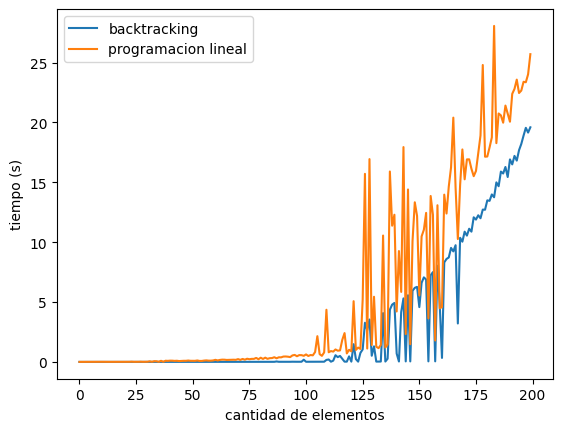
\includegraphics[width=1\textwidth]{img/backvslp.png}
\end{figure}

Backtracking obtiene mejores tiempo de ejecución que programación lineal para
encontrar la solución óptima.

\subsection{Tiempos con algorimo greedy}

\begin{figure}[H]
    \centering
    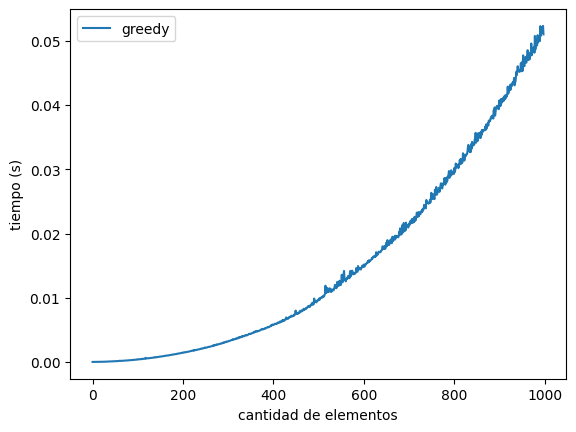
\includegraphics[width=1\textwidth]{img/greedy.png}
\end{figure}

\subsection{Programación Lineal Relajada}

\begin{figure}[H]
    \centering
    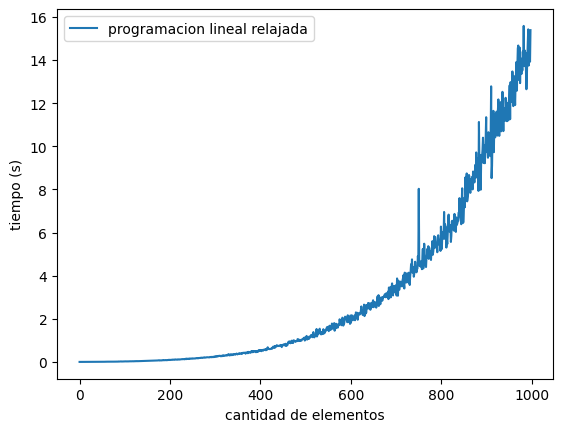
\includegraphics[width=1\textwidth]{img/pl_rlx.png}
\end{figure}

Notar la diferencia de tiempos (eje y) entre greedy y programación lineal.
